\begin{table}
\caption{Overview of assimilation experiments performed.}
\centering
\begin{tabular}{p{2cm}p{2cm}p{6cm}p{4cm}}
	Experiment& Model &  Assimilated Quantities  & Run dates \\
\hline
E1 & WACCM &	none   & 1-30 Oct 2009	\\
E2 & WACCM &	GPS-RO + NNRA$^b$ tropics only & 1-30 Oct 2009	\\
E3 & WACCM &	GPS-RO + NNRA$^b$ whole atmosphere  & 1-30 Oct 2009	\\
E4 & WACCM &	GPS-RO + NNRA$^b$ whole atmosphere +SABER & 1 Jan - 28 Feb 2009\\	
E5 & CAM	&	none &  1 Jan - 28 Feb 2009 \\
E6 & CAM &	$\chi_1$, $\chi_2$, $\Delta$LOD	& 1 Jan - 28 Feb 2009 \\
E7 & CAM &	Temperature	& 1 Jan -31 Jan 2009	\\
E8 & CAM &	Temperature, $\chi_1$, $\chi_2$, $\Delta$LOD	& 1 Jan - 17 Jan 2009\\
\hline
\end{tabular}
\tablenotetext{a}{Experiments performed by \citet{Pedatella2014}}
\tablenotetext{b}{Observations used in the NCEP/NCAR Reanalysis project \citet{Saha2010}, which include radiosonde and aircraft winds and temperatures, plus satellite drift winds.}
\label{tab:expts}
\end{table}
\clearpage

%-------comparison of the WACCM experiments in terms of true error ----
 \begin{figure}
	 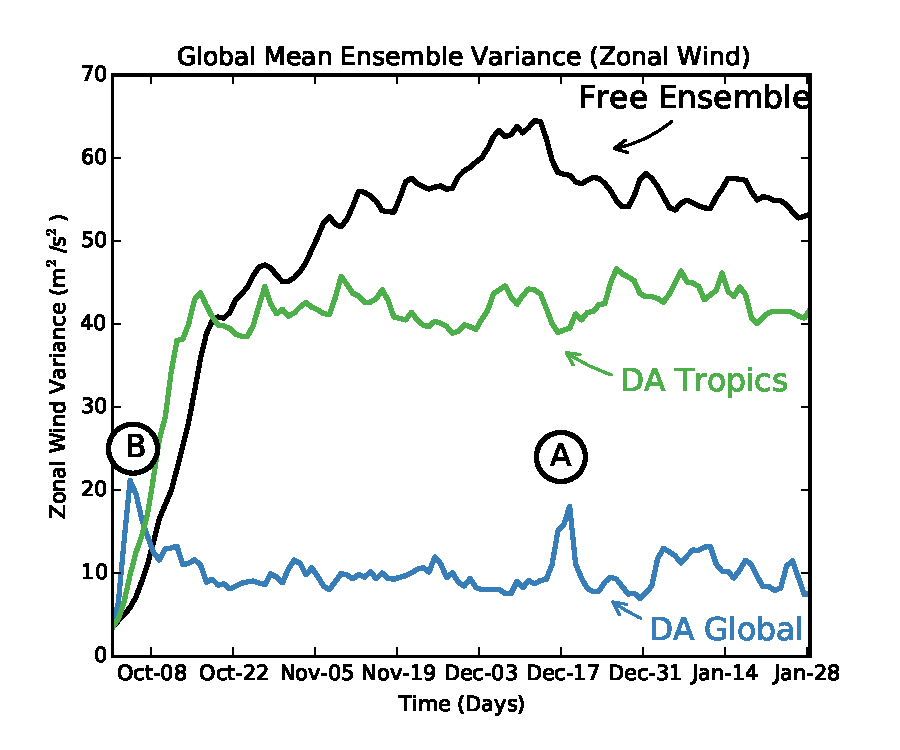
\includegraphics[width=\textwidth]{Paper_figures/ERPDA_paper_evalvariable_state_space.pdf}
	 \caption{Global-average ensemble variance as a function of time, comparing DART-WACCM experiments with increasing observational constrains (Table \ref{tab:expts}).}
	 \label{fig:evalvariable_state}
\end{figure}

%-------comparison of the WACCM experiments in terms of aam ----
\begin{figure}
	 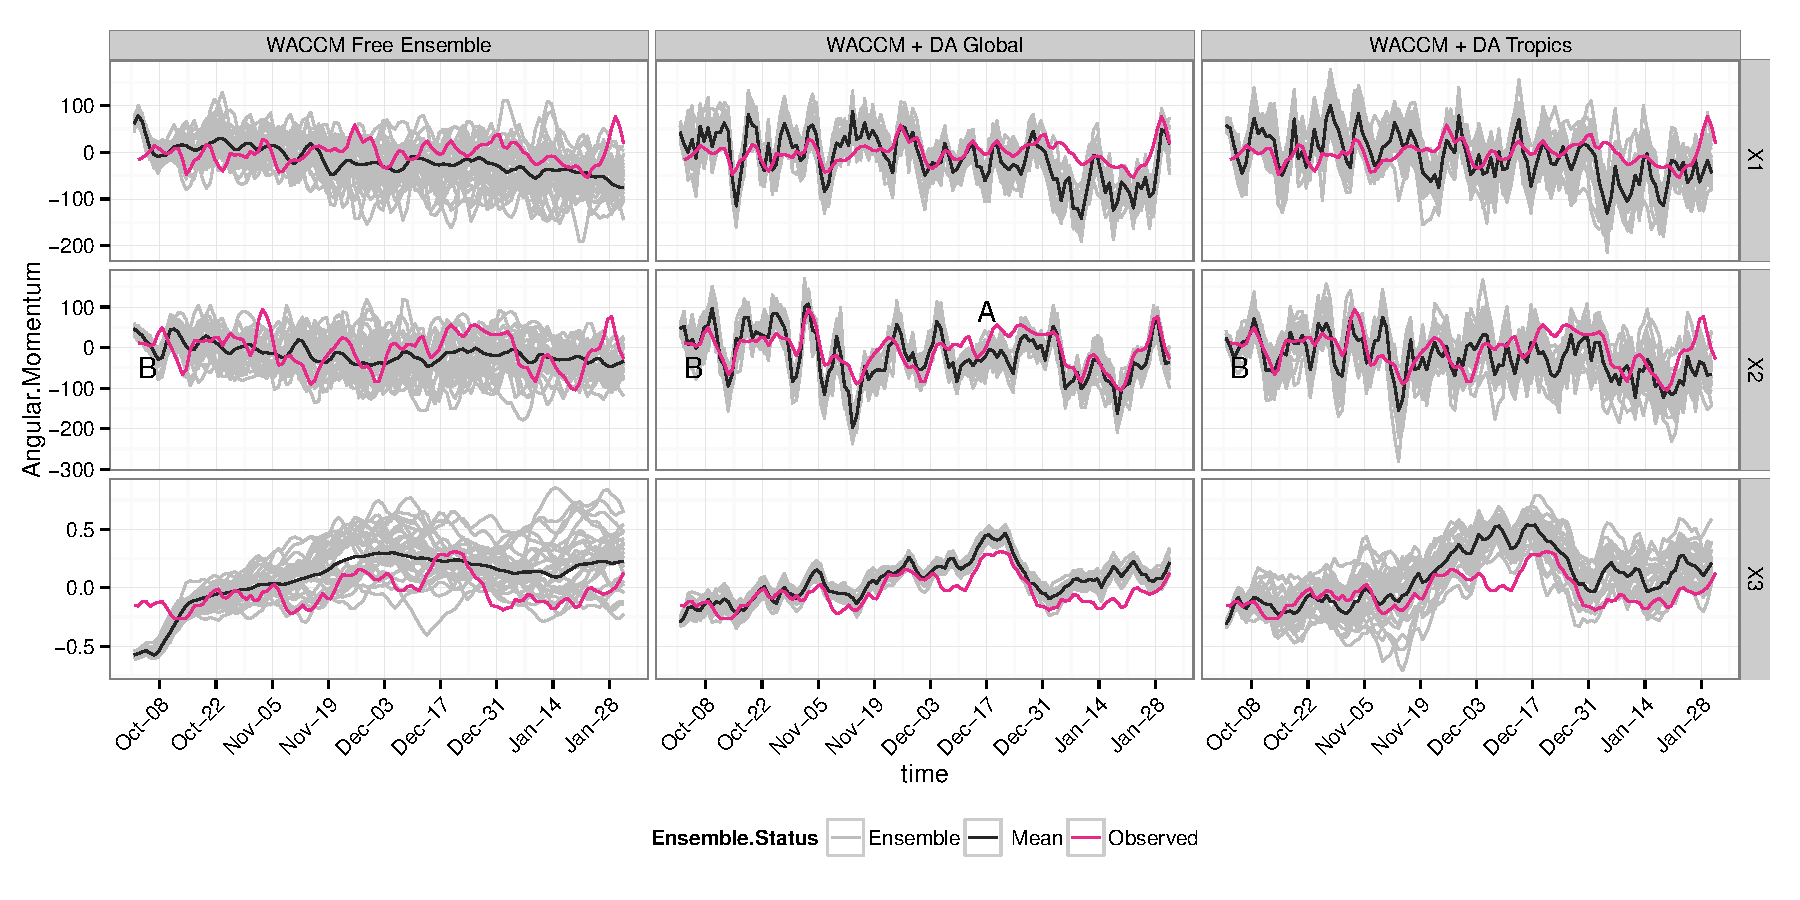
\includegraphics[width=\textwidth]{Paper_figures/ERPDA_paper_evalvariable_aam_space.pdf}
	 \caption{Comparison of the ensemble (gray) in DART-WACCM experiments with increasing observational constrains (Table \ref{tab:expts}), in terms of angular momentum excitation functions $\chi_2$ and $\chi_3$, and compared to the angular momentum implied by the corresponding Earth rotation parameters.}
	 \label{fig:evalvariable_aam}
\end{figure}

%------comparison of the DA runs in the observation space
\begin{figure}[p]
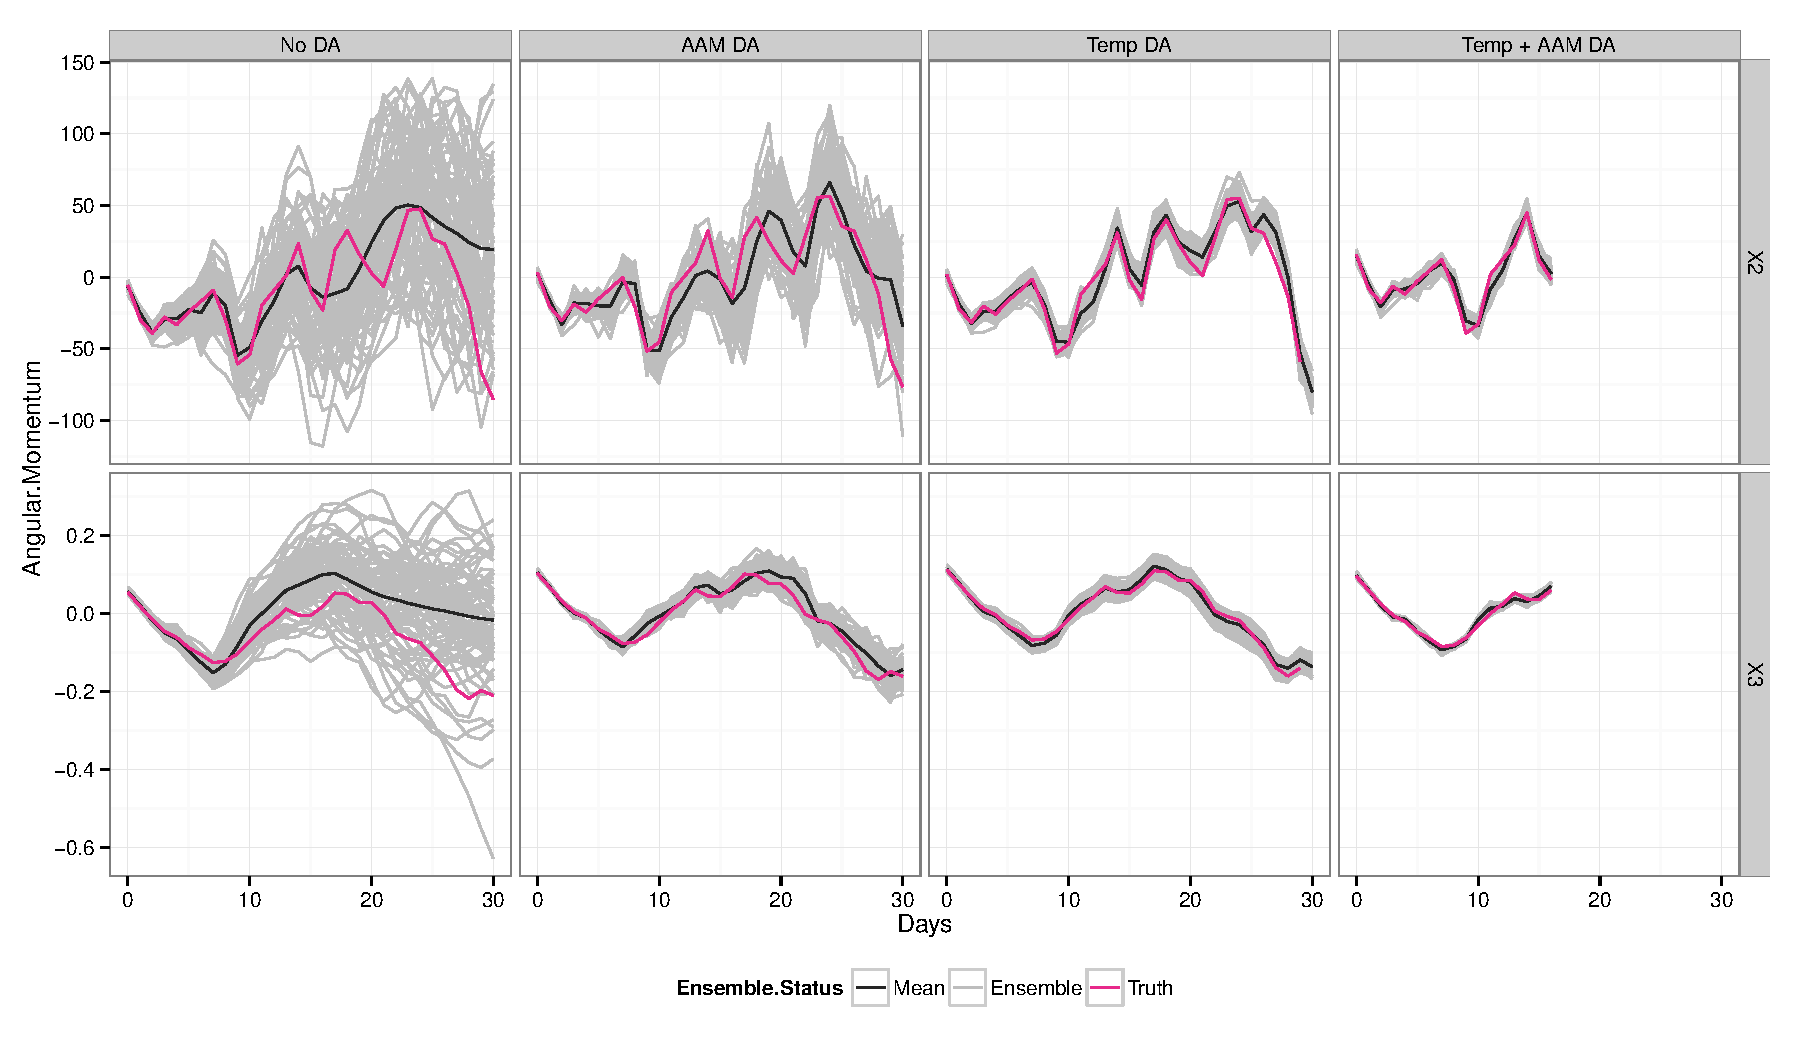
\includegraphics[width=\textwidth]{Paper_figures/ERPDA_paper_erpda_obs_space.pdf} 
\caption{ The DART prior ensemble (gray) compared to the true state (green) in terms of angular momentum components $\chi_2$ and $\chi_3$, comparing four DART-CAM experiments (Table \ref{tab:expts}).  }
 \label{fig:fit_to_ERPs}
\end{figure}

%-----evolution of the covariances between local variables and the AAM observations 
 \begin{figure}
	 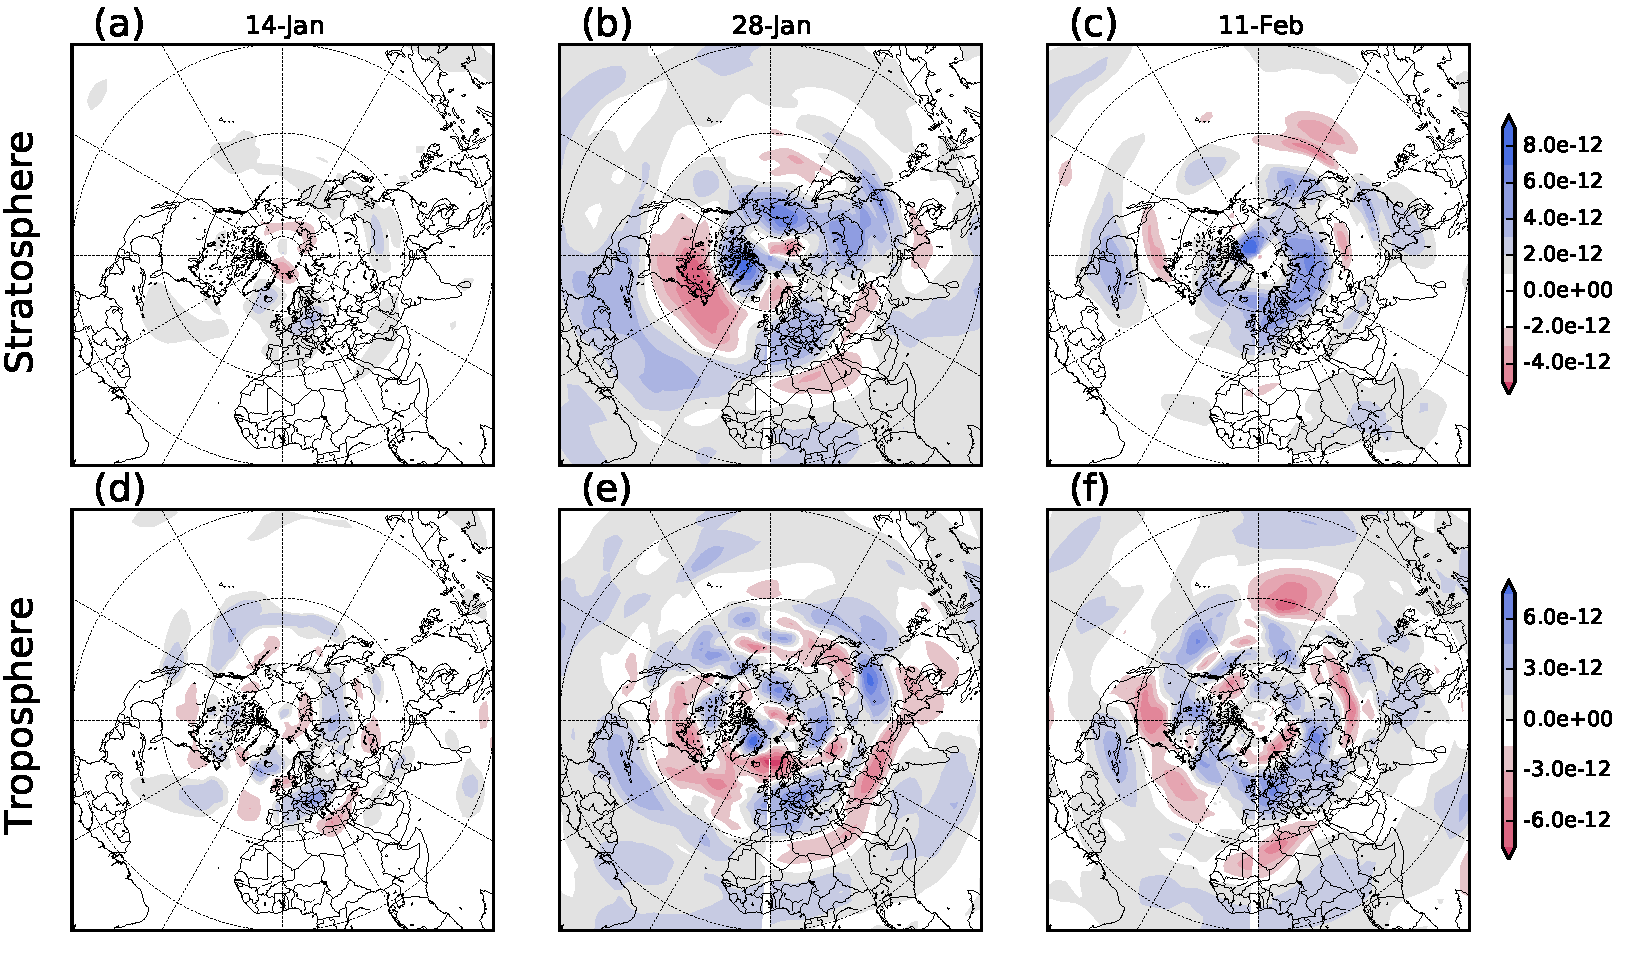
\includegraphics[width=\textwidth]{Paper_figures/ERPDA_paper_U_to_LOD_covariances_.pdf}
	 \caption{Evolution of the covariance between the zonal wind and the axial angular momentum ($\chi_3$) on three dates, assimilating only the three components of angular momentum. The top row shows values averaged over stratospheric levels, while the bottom row shows values averaged over tropospheric levels.}
 \label{fig:covariances}
\end{figure}

%-----evolution of the prior error and corresponding increments 
 \begin{figure}
	 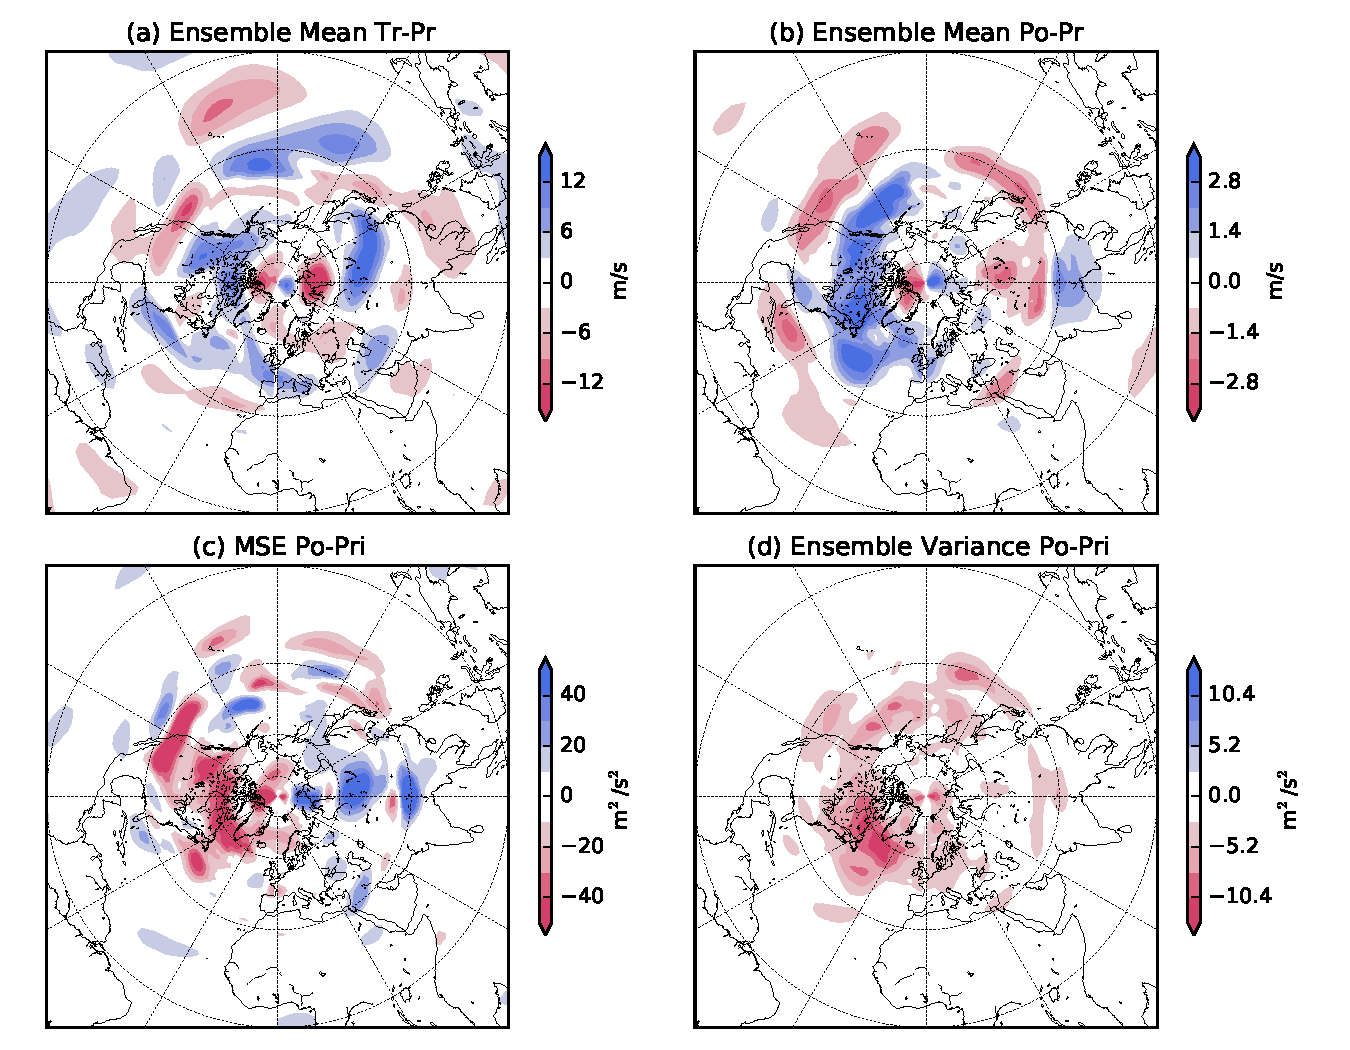
\includegraphics[width=\textwidth]{Paper_figures/ERPDA_paper_U_priorerror_vs_increment_vs_ER_31jan.pdf}
	 \caption{Snapshots of the (a) bias (truth minus prior ensemble mean), (b) analysis increment (posterior minus prior ensemble mean), (c) posterior minus prior mean square error, and (d) posterior-minus prior ensemble variance on 31 January, i.e. after 1 month of assimilation, on the 320 hPa vertical leve, assimilating the three angular momentum components only. } 
 \label{fig:error_increments}
\end{figure}


%-----focus on the ensemble in two regions to show how it is moved away from the true state
 \begin{figure}
	 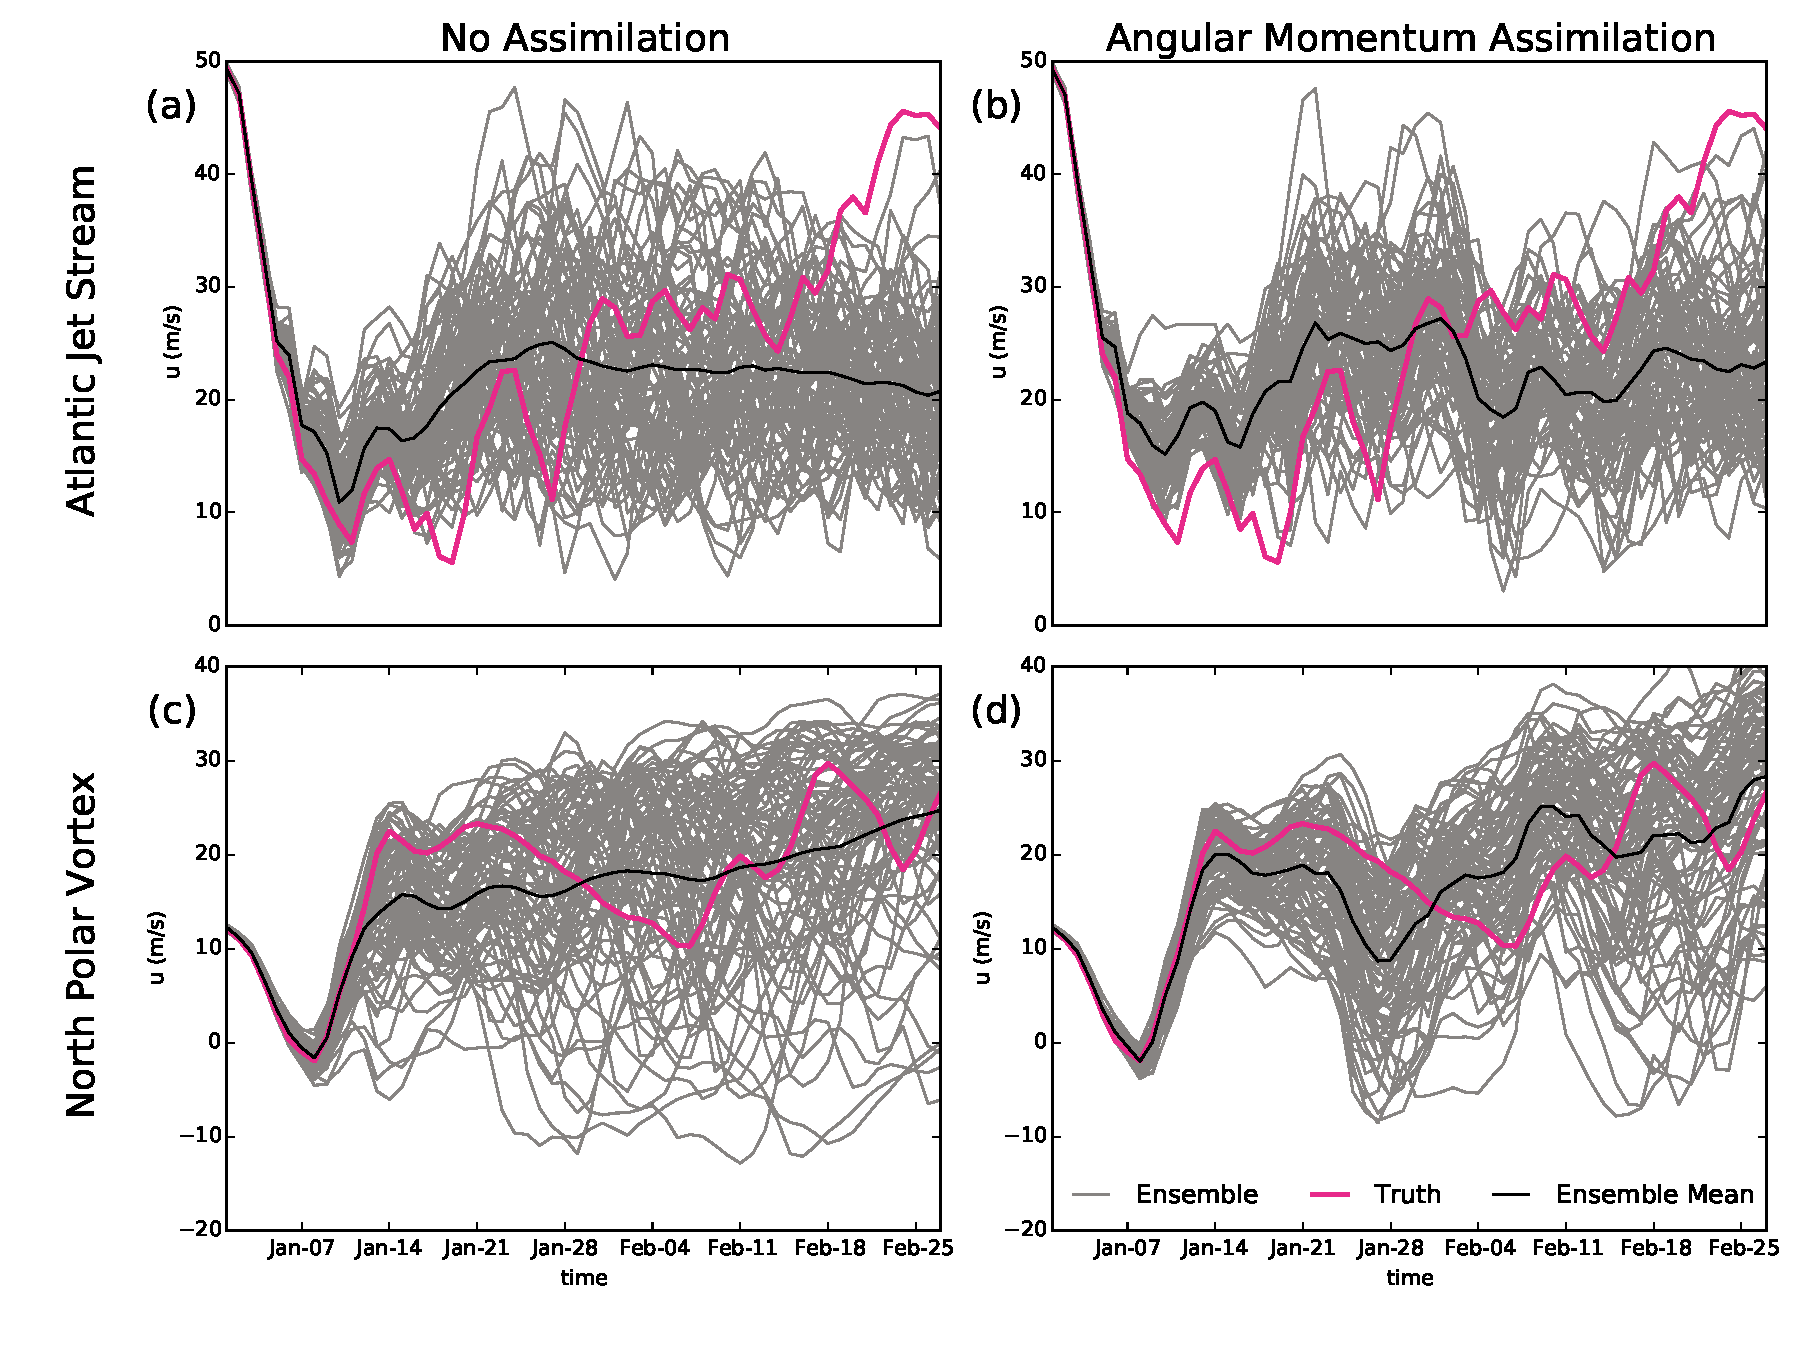
\includegraphics[width=\textwidth]{Paper_figures/ERPDA_paper_point_checks.pdf}
	 \caption{Comparison of the ensemble (gray) and its mean (black) to the true state (pink), for no assimilation [(a) and (c)], and with assimilation of the three angular momentum components [(b) and (d)]. The top row shows zonal wind averaged over the Atlantic jet stream, and the bottom row shows zonal wind averaged in the polar vortex (see text).}
	 \label{fig:point_checks}
\end{figure}




%------MSE increments in time (RST means error reduction) comparing RST and ERPSRT
 \begin{figure}
	 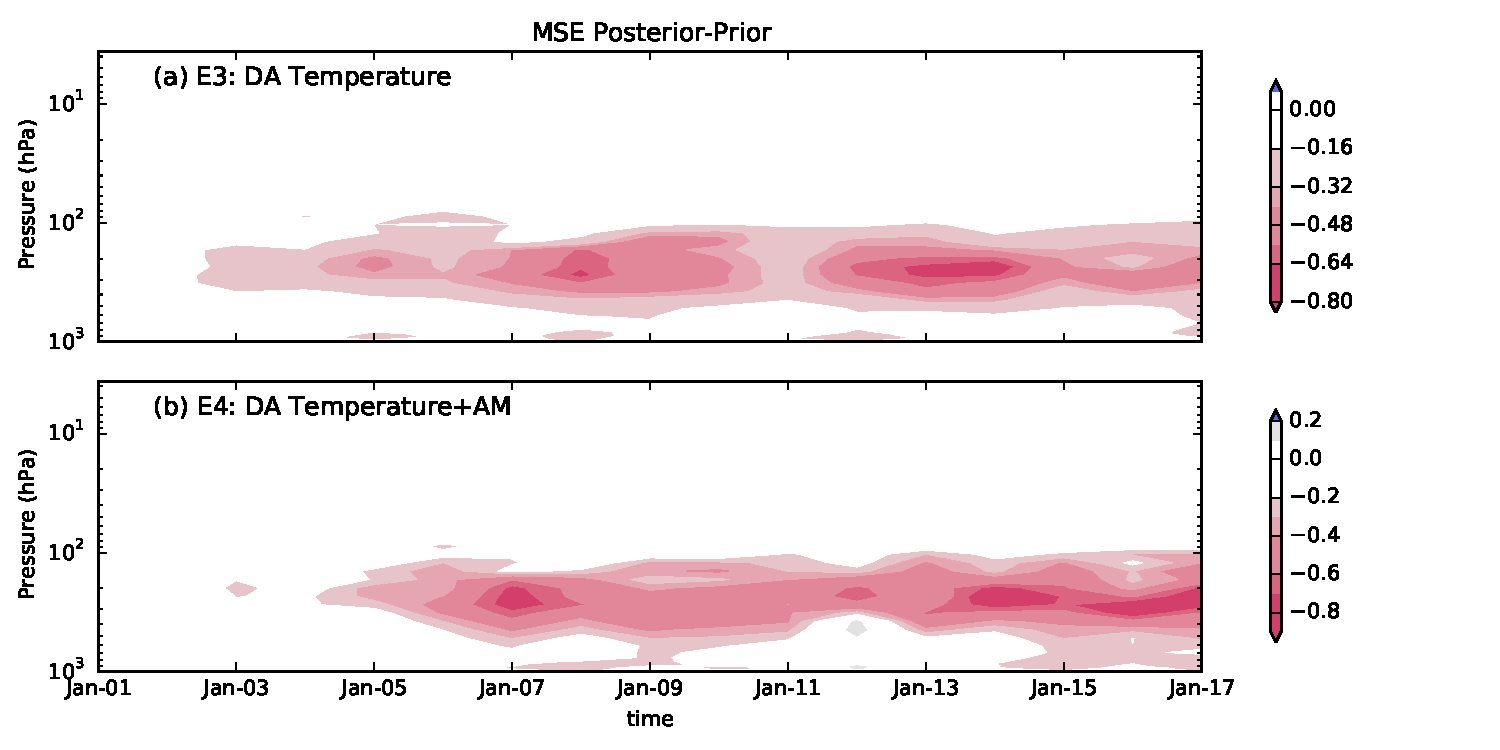
\includegraphics[width=\textwidth]{Paper_figures/ERPDA_paper_MSEincrement_comparison.pdf}
	 \caption{Vertical profiles of the difference in MSE between the posterior and prior states (red means that assimilation reduces error) as a function of time, (a) assimilating a global grid of temperatures, and (b) additionally assimilating the three global angular momentum components.}
	 \label{fig:added_value_MSEincrement}
\end{figure}


%------MSE diff between ERPRST and RST (red is good)
 \begin{figure}
	 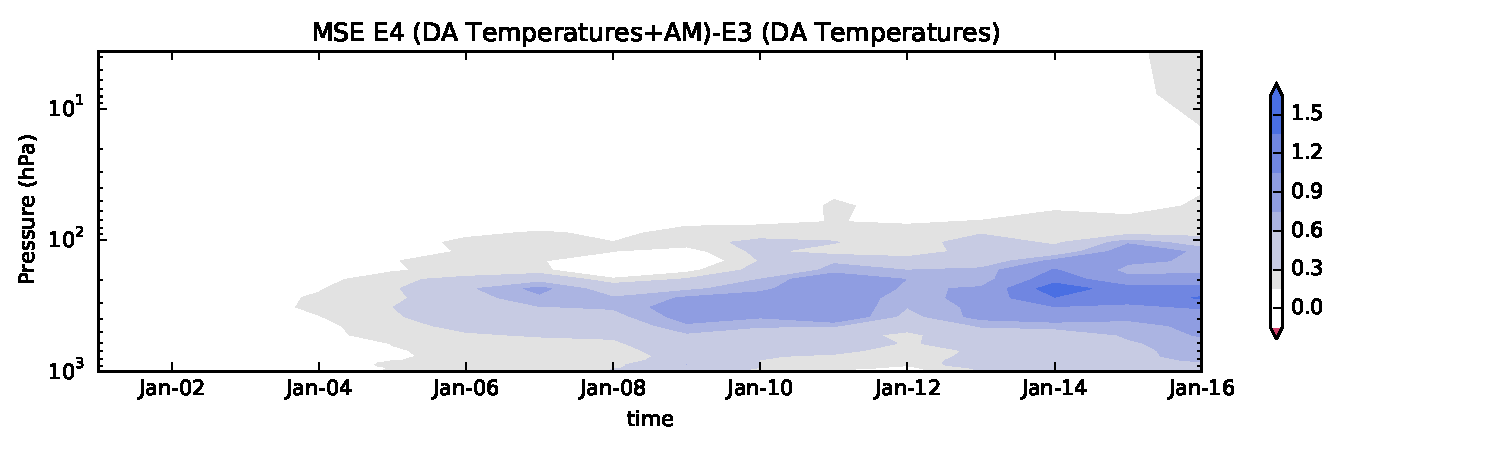
\includegraphics[width=\textwidth]{Paper_figures/ERPDA_paper_MSE_RST_vs_ERPRST.pdf}
	 \caption{Vertical profiles of the differenence in MSE between assimilation of temperatures and global angular momentum, and assimilation of temperatures only. Blue indicates that the error is higher when angular momentum observations are added.}
	 \label{fig:added_value_MSE}
\end{figure}
